\PassOptionsToPackage{unicode=true}{hyperref} % options for packages loaded elsewhere
\PassOptionsToPackage{hyphens}{url}
%
\documentclass[
]{article}
\usepackage{lmodern}
\usepackage{amssymb,amsmath}
\usepackage{ifxetex,ifluatex}
\ifnum 0\ifxetex 1\fi\ifluatex 1\fi=0 % if pdftex
  \usepackage[T1]{fontenc}
  \usepackage[utf8]{inputenc}
  \usepackage{textcomp} % provides euro and other symbols
\else % if luatex or xelatex
  \usepackage{unicode-math}
  \defaultfontfeatures{Scale=MatchLowercase}
  \defaultfontfeatures[\rmfamily]{Ligatures=TeX,Scale=1}
\fi
% use upquote if available, for straight quotes in verbatim environments
\IfFileExists{upquote.sty}{\usepackage{upquote}}{}
\IfFileExists{microtype.sty}{% use microtype if available
  \usepackage[]{microtype}
  \UseMicrotypeSet[protrusion]{basicmath} % disable protrusion for tt fonts
}{}
\makeatletter
\@ifundefined{KOMAClassName}{% if non-KOMA class
  \IfFileExists{parskip.sty}{%
    \usepackage{parskip}
  }{% else
    \setlength{\parindent}{0pt}
    \setlength{\parskip}{6pt plus 2pt minus 1pt}}
}{% if KOMA class
  \KOMAoptions{parskip=half}}
\makeatother
\usepackage{xcolor}
\IfFileExists{xurl.sty}{\usepackage{xurl}}{} % add URL line breaks if available
\IfFileExists{bookmark.sty}{\usepackage{bookmark}}{\usepackage{hyperref}}
\hypersetup{
  pdftitle={Exponential Distribution Comparison to the Centeral Limit Theorem},
  pdfauthor={Alex MacCalman},
  pdfborder={0 0 0},
  breaklinks=true}
\urlstyle{same}  % don't use monospace font for urls
\usepackage[margin=1in]{geometry}
\usepackage{color}
\usepackage{fancyvrb}
\newcommand{\VerbBar}{|}
\newcommand{\VERB}{\Verb[commandchars=\\\{\}]}
\DefineVerbatimEnvironment{Highlighting}{Verbatim}{commandchars=\\\{\}}
% Add ',fontsize=\small' for more characters per line
\usepackage{framed}
\definecolor{shadecolor}{RGB}{248,248,248}
\newenvironment{Shaded}{\begin{snugshade}}{\end{snugshade}}
\newcommand{\AlertTok}[1]{\textcolor[rgb]{0.94,0.16,0.16}{#1}}
\newcommand{\AnnotationTok}[1]{\textcolor[rgb]{0.56,0.35,0.01}{\textbf{\textit{#1}}}}
\newcommand{\AttributeTok}[1]{\textcolor[rgb]{0.77,0.63,0.00}{#1}}
\newcommand{\BaseNTok}[1]{\textcolor[rgb]{0.00,0.00,0.81}{#1}}
\newcommand{\BuiltInTok}[1]{#1}
\newcommand{\CharTok}[1]{\textcolor[rgb]{0.31,0.60,0.02}{#1}}
\newcommand{\CommentTok}[1]{\textcolor[rgb]{0.56,0.35,0.01}{\textit{#1}}}
\newcommand{\CommentVarTok}[1]{\textcolor[rgb]{0.56,0.35,0.01}{\textbf{\textit{#1}}}}
\newcommand{\ConstantTok}[1]{\textcolor[rgb]{0.00,0.00,0.00}{#1}}
\newcommand{\ControlFlowTok}[1]{\textcolor[rgb]{0.13,0.29,0.53}{\textbf{#1}}}
\newcommand{\DataTypeTok}[1]{\textcolor[rgb]{0.13,0.29,0.53}{#1}}
\newcommand{\DecValTok}[1]{\textcolor[rgb]{0.00,0.00,0.81}{#1}}
\newcommand{\DocumentationTok}[1]{\textcolor[rgb]{0.56,0.35,0.01}{\textbf{\textit{#1}}}}
\newcommand{\ErrorTok}[1]{\textcolor[rgb]{0.64,0.00,0.00}{\textbf{#1}}}
\newcommand{\ExtensionTok}[1]{#1}
\newcommand{\FloatTok}[1]{\textcolor[rgb]{0.00,0.00,0.81}{#1}}
\newcommand{\FunctionTok}[1]{\textcolor[rgb]{0.00,0.00,0.00}{#1}}
\newcommand{\ImportTok}[1]{#1}
\newcommand{\InformationTok}[1]{\textcolor[rgb]{0.56,0.35,0.01}{\textbf{\textit{#1}}}}
\newcommand{\KeywordTok}[1]{\textcolor[rgb]{0.13,0.29,0.53}{\textbf{#1}}}
\newcommand{\NormalTok}[1]{#1}
\newcommand{\OperatorTok}[1]{\textcolor[rgb]{0.81,0.36,0.00}{\textbf{#1}}}
\newcommand{\OtherTok}[1]{\textcolor[rgb]{0.56,0.35,0.01}{#1}}
\newcommand{\PreprocessorTok}[1]{\textcolor[rgb]{0.56,0.35,0.01}{\textit{#1}}}
\newcommand{\RegionMarkerTok}[1]{#1}
\newcommand{\SpecialCharTok}[1]{\textcolor[rgb]{0.00,0.00,0.00}{#1}}
\newcommand{\SpecialStringTok}[1]{\textcolor[rgb]{0.31,0.60,0.02}{#1}}
\newcommand{\StringTok}[1]{\textcolor[rgb]{0.31,0.60,0.02}{#1}}
\newcommand{\VariableTok}[1]{\textcolor[rgb]{0.00,0.00,0.00}{#1}}
\newcommand{\VerbatimStringTok}[1]{\textcolor[rgb]{0.31,0.60,0.02}{#1}}
\newcommand{\WarningTok}[1]{\textcolor[rgb]{0.56,0.35,0.01}{\textbf{\textit{#1}}}}
\usepackage{graphicx,grffile}
\makeatletter
\def\maxwidth{\ifdim\Gin@nat@width>\linewidth\linewidth\else\Gin@nat@width\fi}
\def\maxheight{\ifdim\Gin@nat@height>\textheight\textheight\else\Gin@nat@height\fi}
\makeatother
% Scale images if necessary, so that they will not overflow the page
% margins by default, and it is still possible to overwrite the defaults
% using explicit options in \includegraphics[width, height, ...]{}
\setkeys{Gin}{width=\maxwidth,height=\maxheight,keepaspectratio}
\setlength{\emergencystretch}{3em}  % prevent overfull lines
\providecommand{\tightlist}{%
  \setlength{\itemsep}{0pt}\setlength{\parskip}{0pt}}
\setcounter{secnumdepth}{-2}
% Redefines (sub)paragraphs to behave more like sections
\ifx\paragraph\undefined\else
  \let\oldparagraph\paragraph
  \renewcommand{\paragraph}[1]{\oldparagraph{#1}\mbox{}}
\fi
\ifx\subparagraph\undefined\else
  \let\oldsubparagraph\subparagraph
  \renewcommand{\subparagraph}[1]{\oldsubparagraph{#1}\mbox{}}
\fi

% set default figure placement to htbp
\makeatletter
\def\fps@figure{htbp}
\makeatother


\title{Exponential Distribution Comparison to the Centeral Limit Theorem}
\author{Alex MacCalman}
\date{5/14/2020}

\begin{document}
\maketitle

\hypertarget{overview}{%
\section{Overview}\label{overview}}

In this project we will investigate the exponential distribution in R
and compare it with the Central Limit Theorem. The mean of exponential
distribution is 1/lambda and the standard deviation is also 1/lambda. We
will set lambda = 0.2 for all of the simulations. We ill investigate the
distribution of averages of 40 exponentials. \# Simulation First we run
a simulation, then calcualte the sample mean and variance and
theoretcial mean and variance.

\begin{Shaded}
\begin{Highlighting}[]
\NormalTok{lambda <-}\StringTok{ }\FloatTok{0.2}
\NormalTok{n <-}\StringTok{ }\DecValTok{40}
\NormalTok{B <-}\StringTok{ }\DecValTok{1000}
\KeywordTok{set.seed}\NormalTok{(}\DecValTok{10}\NormalTok{)}
\NormalTok{sim <-}\StringTok{ }\KeywordTok{matrix}\NormalTok{(}\KeywordTok{rexp}\NormalTok{(n}\OperatorTok{*}\NormalTok{B, lambda), B, n)}
\NormalTok{means <-}\StringTok{ }\KeywordTok{apply}\NormalTok{(sim, }\DecValTok{1}\NormalTok{, mean)}
\NormalTok{sampleMean <-}\StringTok{ }\KeywordTok{mean}\NormalTok{(means)}
\NormalTok{theoreticalMean <-}\StringTok{ }\DecValTok{1}\OperatorTok{/}\NormalTok{lambda}
\NormalTok{sampleVar <-}\StringTok{ }\KeywordTok{var}\NormalTok{(means)}
\NormalTok{theoreticalVar <-}\StringTok{ }\NormalTok{(}\DecValTok{1}\OperatorTok{/}\NormalTok{lambda)}\OperatorTok{^}\DecValTok{2}\OperatorTok{/}\NormalTok{n}
\end{Highlighting}
\end{Shaded}

Next we display a histogram of the simulation and compare to the
theoretical mean and variance with the sample mean and variance.

\begin{Shaded}
\begin{Highlighting}[]
\KeywordTok{hist}\NormalTok{(means, }\DataTypeTok{col =} \StringTok{"green"}\NormalTok{, }\DataTypeTok{breaks =} \DecValTok{30}\NormalTok{, }\DataTypeTok{main =} \StringTok{"Histogram of exponential random variants with lambda = 0.2"}\NormalTok{, }\DataTypeTok{xlab =} \StringTok{"Sample Means of 40 Replications"}\NormalTok{)}
\KeywordTok{text}\NormalTok{(}\DecValTok{7}\NormalTok{,}\DecValTok{80}\NormalTok{, }\KeywordTok{paste}\NormalTok{(}\StringTok{"Sample Mean = "}\NormalTok{, }\KeywordTok{round}\NormalTok{(sampleMean, }\DecValTok{4}\NormalTok{), }\StringTok{"}\CharTok{\textbackslash{}n}\StringTok{ Theorectical Mean ="}\NormalTok{, theoreticalMean, }\StringTok{"}\CharTok{\textbackslash{}n}\StringTok{"}\NormalTok{, }\StringTok{"}\CharTok{\textbackslash{}n}\StringTok{ Sample Variance = "}\NormalTok{, }\KeywordTok{round}\NormalTok{(sampleVar, }\DecValTok{4}\NormalTok{), }\StringTok{"}\CharTok{\textbackslash{}n}\StringTok{ Theorectical Variance ="}\NormalTok{, theoreticalVar))}
\end{Highlighting}
\end{Shaded}

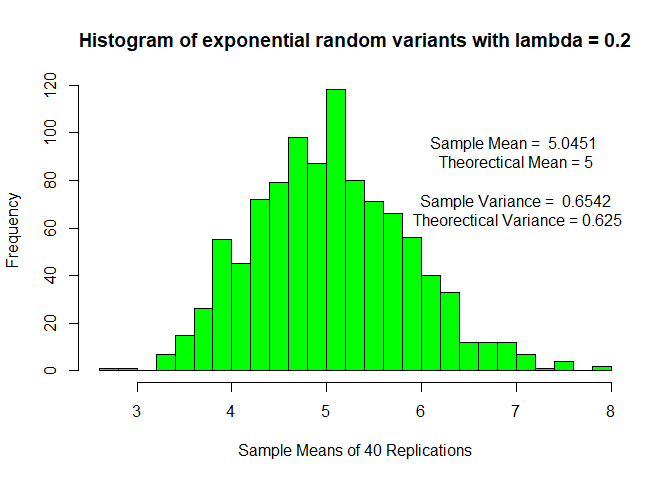
\includegraphics{Exponential-Sample_files/figure-latex/unnamed-chunk-2-1.pdf}

In order to show that the distribution is approximatly normal, we
overlay a density plot.

\begin{Shaded}
\begin{Highlighting}[]
\KeywordTok{hist}\NormalTok{(means, }\DataTypeTok{col =} \StringTok{"blue"}\NormalTok{, }\DataTypeTok{breaks =} \DecValTok{30}\NormalTok{, }\DataTypeTok{main =} \StringTok{"Histogram of exponential random variants compared with normal"}\NormalTok{, }\DataTypeTok{xlab =} \StringTok{"Sample Means of 40 Replications"}\NormalTok{, }\DataTypeTok{prob =} \OtherTok{TRUE}\NormalTok{)}
\KeywordTok{lines}\NormalTok{(}\KeywordTok{density}\NormalTok{(means), }\DataTypeTok{col =} \StringTok{"red"}\NormalTok{)}
\end{Highlighting}
\end{Shaded}

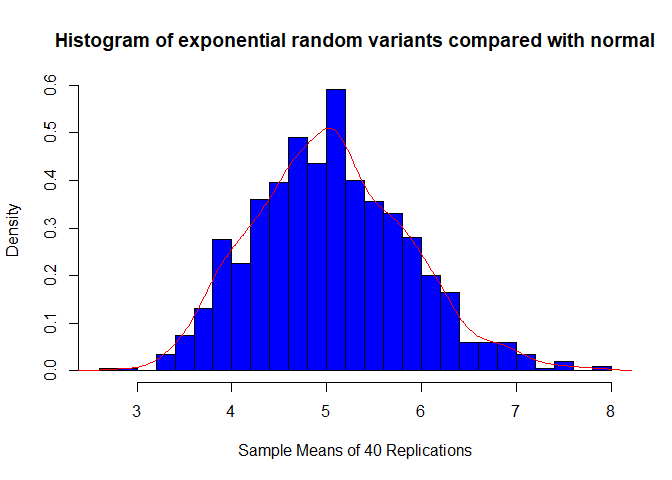
\includegraphics{Exponential-Sample_files/figure-latex/unnamed-chunk-3-1.pdf}

Now we will calculate a 95\% confidence interval for the exponential
sample mean.

\begin{Shaded}
\begin{Highlighting}[]
\KeywordTok{t.test}\NormalTok{(means)}\OperatorTok{$}\NormalTok{conf.int}
\end{Highlighting}
\end{Shaded}

\begin{verbatim}
## [1] 4.994869 5.095250
## attr(,"conf.level")
## [1] 0.95
\end{verbatim}

\end{document}
